\chapter{Messagers chimiques et transduction du signal}\label{ch:b2:cell-signalling}

Une molécule d'adrénaline qui arrive à la surface d'une cellule du foie
n'y entre jamais. Elle se fixe sur une protéine à l'extérieur, en modifie
la forme, et en une seconde la cellule a fabriqué dix mille molécules
d'un \omterm{prop:b2:cell-signalling:gpcr}{second messager}, activé cent mille molécules d'enzyme et commencé à
libérer un million de molécules de glucose --- une chaîne
d'amplifications d'un facteur un million, déclenchée par un signal resté
à la porte. Ce chapitre traite des messagers que les cellules
s'échangent et de la manière dont une cellule convertit un message reçu
à sa surface en une modification de sa chimie, de ses gènes ou de sa
forme~: les récepteurs, les \omterm{prop:b2:cell-signalling:gpcr}{seconds messagers}, les cascades de kinases,
et les deux modèles --- la signalisation rapide et câblée des nerfs et la
signalisation lente et diffusée des \omterm{def:b2:cell-signalling:kinds}{hormones} --- dont le contraste
traverse toute la suite de ce livre.

\section{Les messagers}

\begin{definition}[Les types de communication chimique]\label{def:b2:cell-signalling:kinds}
\index{hormone}\index{communication endocrine}\index{communication paracrine}\index{neurotransmetteur}
Une cellule communique avec une autre au moyen d'une molécule sécrétée,
un \emph{messager} ou \emph{ligand}, qui se fixe sur un \emph{récepteur}
situé à la surface ou à l'intérieur de la cible. Selon la portée~: la
communication \emph{endocrine}, dans laquelle une \emph{hormone} est
libérée dans le \omterm{def:b2:blood-circulation:blood}{sang} par une glande et atteint toutes les cellules du
corps, n'agissant que sur celles qui portent le récepteur, en quelques
minutes à quelques heures (insuline, cortisol, adrénaline, thyroxine)~;
la communication \emph{paracrine}, dans laquelle le messager diffuse
jusqu'aux cellules voisines, à moins d'un millimètre, et est détruit en
chemin (facteurs de croissance, histamine, prostaglandines, morphogènes
du \cref{ch:b2:vertebrate-development})~; la communication
\emph{autocrine}, par laquelle la cellule s'adresse à elle-même~; et la
communication \emph{synaptique}, dans laquelle un neurone libère un
\emph{neurotransmetteur} à travers un espace de \qty{20}{nm} sur une
seule cellule cible, en une milliseconde
(\cref{ch:b2:neurons-synapses}). Selon la chimie~: les messagers
\emph{hydrosolubles} --- dérivés d'acides aminés comme l'adrénaline,
peptides et protéines comme l'insuline --- ne peuvent pas traverser la
membrane et agissent sur des récepteurs de surface~; les messagers
\emph{liposolubles} --- les stéroïdes (cortisol, œstradiol,
testostérone), la thyroxine, l'acide rétinoïque, le monoxyde d'azote ---
la traversent et agissent sur des récepteurs intérieurs. Les systèmes
endocrinien et nerveux sont les deux manières dont un corps de
$10^{13}$ cellules se coordonne~: l'un diffuse lentement à tous, l'autre
câble rapidement vers quelqu'un.
\end{definition}

\begin{omfigure}
\begin{tikzpicture}[every node/.style={font=\scriptsize}, >=stealth]
  % endocrine
  \begin{scope}
    \draw[thick, fill=omProp!25] (0,1.6) circle (0.35); \node[above] at (0,2.0) {glande};
    \draw[very thick, omThm!60] (-0.5,0.6) -- (4.5,0.6); \draw[very thick, omThm!60] (-0.5,0.2) -- (4.5,0.2); \node[omThm!70!black] at (2,0.4) {sang};
    \foreach \x in {0.6,1.5,2.4,3.3} \fill[omProp] (\x,0.4) circle (0.05);
    \draw[->, omProp] (0,1.25) -- (0,0.65);
    \draw[thick, fill=omDef!20] (3.8,-0.8) circle (0.35); \node[below, align=center] at (3.8,-1.2) {cellule cible\\porteuse du récepteur};
    \draw[->, omProp] (3.8,0.15) -- (3.8,-0.4);
    \draw[thick, fill=gray!20] (1.0,-0.8) circle (0.35); \node[below, align=center] at (1.0,-1.2) {sans récepteur~:\\l'ignore};
    \node[align=center] at (2.2,-2.4) {endocrine~: hormone dans le sang,\\corps entier, minutes à heures};
  \end{scope}
  % paracrine
  \begin{scope}[xshift=6.6cm]
    \draw[thick, fill=omProp!25] (0.8,0.6) circle (0.35);
    \foreach \a in {0,45,...,315} \fill[omProp] (0.8,0.6) ++(\a:0.6) circle (0.04);
    \draw[thick, fill=omDef!20] (1.9,0.9) circle (0.3); \draw[thick, fill=omDef!20] (1.7,-0.2) circle (0.3); \draw[thick, fill=omDef!20] (-0.2,0.0) circle (0.3);
    \node[align=center] at (0.8,-2.4) {paracrine~: diffuse vers\\les voisines, détruit\\en moins d'un millimètre};
  \end{scope}
  % synaptic
  \begin{scope}[xshift=11.6cm]
    \draw[very thick, omDef] (0,1.8) -- (0,0.5); \draw[thick, fill=omDef!25] (0,0.3) circle (0.25);
    \draw[thick, fill=omExo!30] (0,-0.5) circle (0.3);
    \foreach \x in {-0.08,0,0.08} \fill[omProp] (\x,-0.05) circle (0.03);
    \node[align=center] at (0.2,-2.4) {synaptique~: une cible,\\\qty{20}{nm},\\une milliseconde};
  \end{scope}
\end{tikzpicture}

{\small Trois portées de la communication chimique~: une \omterm{def:b2:cell-signalling:kinds}{hormone} diffusée
par le \omterm{def:b2:blood-circulation:blood}{sang} à toutes les cellules qui portent son récepteur~; un facteur
paracrine qui atteint ses voisines~; un \omterm{def:b2:cell-signalling:kinds}{neurotransmetteur} délivré à une
seule cellule à travers une synapse.}
\end{omfigure}

\begin{theorem}[Le taux d'occupation des récepteurs]\label{thm:b2:cell-signalling:occupancy}
\index{constante de dissociation}\index{taux d'occupation des recepteurs@taux d'occupation des récepteurs}
Un récepteur $R$ fixe son ligand $L$ de façon réversible, $R + L
\rightleftharpoons RL$, avec une \emph{\omterm{thm:b2:cell-signalling:occupancy}{constante de dissociation}} $K_d =
[R][L]/[RL]$. À l'équilibre, la fraction des récepteurs occupés vaut
\[
\theta = \frac{[RL]}{[R]_{\text{tot}}} = \frac{[L]}{K_d + [L]},
\]
la même hyperbole que la saturation d'une enzyme. $K_d$ est la
concentration pour laquelle la moitié des récepteurs est occupée et
mesure l'\emph{affinité}~: plus il est faible, plus la liaison est
forte. Les récepteurs hormonaux ont des $K_d$ de l'ordre du nanomolaire
au picomolaire, accordés aux concentrations auxquelles circulent les
\omterm{def:b2:cell-signalling:kinds}{hormones} ($10^{-12}$ à
$10^{-9}$ mol/L)~: pour $[L] = K_d/10$, un dixième des récepteurs sont
occupés, pour
$10K_d$, neuf dixièmes. Une cellule ne peut pas répondre à une \omterm{def:b2:cell-signalling:kinds}{hormone}
dont elle ne possède pas les récepteurs, et elle règle sa sensibilité en
modifiant le nombre de ses récepteurs, ou --- comme au
\cref{ch:b2:reproductive-hormones} --- en les retirant lorsque l'\omterm{def:b2:cell-signalling:kinds}{hormone}
est présente en permanence.
\end{theorem}
\begin{proof}
Avec $[R] = [R]_{\text{tot}} - [RL]$, $K_d = ([R]_{\text{tot}} -
[RL])[L]/[RL]$, donc $[RL](K_d + [L]) = [R]_{\text{tot}}[L]$, ce qui
donne la formule. C'est l'expression de Michaelis--Menten du volume de
première année, sans l'étape catalytique.
\end{proof}

\begin{omfigure}
\begin{tikzpicture}
\begin{axis}[
  width=0.68\linewidth, height=5.2cm,
  axis x line=bottom, axis y line=left,
  xmode=log, xmin=0.01, xmax=100, ymin=0, ymax=1.1,
  xlabel={concentration du ligand (en unités de $K_d$)}, ylabel={fraction des récepteurs occupés},
  xlabel style={font=\small, at={(axis description cs:0.5,-0.13)}, anchor=north},
  ylabel style={font=\small},
  tick label style={font=\small}, xtick={0.01,0.1,1,10,100}, ytick={0,0.5,1},
  clip=false,
]
\addplot[very thick, omDef, domain=0.01:100, samples=100] {x/(1+x)};
\draw[dashed, gray] (axis cs:1,0) -- (axis cs:1,0.5) -- (axis cs:0.01,0.5);
\node[font=\scriptsize, anchor=north west] at (axis cs:1.1,0.48) {$[L] = K_d$~: moitié occupée};
\node[font=\scriptsize, anchor=south east] at (axis cs:0.1,0.1) {10\% à $K_d/10$};
\node[font=\scriptsize, anchor=north west] at (axis cs:10,0.92) {90\% à $10\,K_d$};
\end{axis}
\end{tikzpicture}

{\small Le \omterm{thm:b2:cell-signalling:occupancy}{taux d'occupation des récepteurs} en fonction de la concentration
du ligand, en échelle logarithmique~: la réponse d'une cellule passe d'un
dixième à neuf dixièmes sur une gamme de concentrations d'un facteur
cent centrée sur $K_d$.}
\end{omfigure}

\section{Les récepteurs de surface}

\begin{proposition}[Récepteurs couplés aux protéines G et AMP cyclique]\label{prop:b2:cell-signalling:gpcr}
\index{proteine G@protéine G}\index{recepteur couple aux proteines G@récepteur couplé aux protéines G}\index{AMP cyclique}\index{second messager}\index{proteine kinase A@protéine kinase A}
La plus grande famille de récepteurs --- quelque \num{800} gènes chez
l'être humain, pour des \omterm{def:b2:cell-signalling:kinds}{hormones}, des \omterm{def:b2:cell-signalling:kinds}{neurotransmetteurs}, des odeurs, la
lumière --- est formée de protéines qui traversent sept fois la
membrane. Un ligand qui se fixe à l'extérieur modifie leur forme à
l'intérieur, où elles activent une \emph{\omterm{prop:b2:cell-signalling:gpcr}{protéine G}}~: un interrupteur à
trois sous-unités qui échange son GDP contre du GTP, se dissocie et, sous
sa forme liée au GTP, règle une enzyme effectrice pendant quelques
secondes avant d'hydrolyser le GTP et de s'éteindre d'elle-même.
L'effecteur classique est l'\emph{adénylate cyclase}, qui fabrique
l'\emph{\omterm{prop:b2:cell-signalling:gpcr}{AMP cyclique}} à partir d'ATP~: un petit \emph{\omterm{prop:b2:cell-signalling:gpcr}{second messager}}
diffusible dont la concentration passe en quelques secondes de
\qty{0.1}{\micro mol/L} à plusieurs micromoles par litre, et qui active la
\emph{\omterm{prop:b2:cell-signalling:gpcr}{protéine kinase A}}, une enzyme qui phosphoryle --- et donc active
ou inhibe --- des dizaines de protéines cibles. Le signal prend fin sous
l'action de la phosphodiestérase, qui détruit l'AMPc, et des
phosphatases, qui retirent les phosphates. L'adrénaline agit ainsi sur
une cellule du foie~: récepteur $\to$ \omterm{prop:b2:cell-signalling:gpcr}{protéine G}
$\to$ cyclase $\to$ AMPc $\to$ kinase A $\to$ phosphorylase kinase
$\to$ glycogène phosphorylase $\to$ glucose. Le glucagon emprunte la
même voie~; d'autres \omterm{prop:b2:cell-signalling:gpcr}{protéines G} inhibent la cyclase, ou activent la
phospholipase C, qui libère deux autres \omterm{prop:b2:cell-signalling:gpcr}{seconds messagers},
l'\emph{inositol trisphosphate} --- qui ouvre les réserves de calcium ---
et le diacylglycérol.
\end{proposition}
\begin{proof}[Faits expérimentaux]
Sutherland (1957) montra que l'adrénaline ajoutée à un homogénat de foie
ne libérait du glucose qu'en présence de membranes, que ces membranes
produisaient un facteur thermostable qui activait à lui seul la
phosphorylase dans la fraction dépourvue de membranes, et que ce facteur
était l'\omterm{prop:b2:cell-signalling:gpcr}{AMP cyclique} --- le premier \omterm{prop:b2:cell-signalling:gpcr}{second messager}, et la première
démonstration qu'une \omterm{def:b2:cell-signalling:kinds}{hormone} agit à la surface de la cellule par un
intermédiaire intracellulaire. Rodbell et Gilman (années 1970)
découvrirent que la cyclase avait besoin de GTP et isolèrent la \omterm{prop:b2:cell-signalling:gpcr}{protéine
G} qui transmet le signal du récepteur à l'enzyme~; la toxine cholérique,
qui bloque la \omterm{prop:b2:cell-signalling:gpcr}{protéine G} dans son état actif, fait sécréter par
l'intestin des litres de liquide par jour --- la maladie est un défaut de
signalisation.
\end{proof}

\begin{omfigure}
\begin{tikzpicture}[every node/.style={font=\scriptsize}, >=stealth]
  % membrane
  \fill[omExo!30] (0,2.0) rectangle (12,2.5);
  \node[anchor=east] at (-0.1,2.25) {membrane};
  % receptor
  \draw[thick, fill=omDef!40] (1.0,1.7) rectangle (1.8,2.8); \node[anchor=east] at (0.95,2.65) {récepteur};
  \fill[omProp] (1.4,3.35) circle (0.12); \node[omProp, above] at (1.4,3.45) {adrénaline};
  \draw[->, omProp] (1.4,3.23) -- (1.4,2.85);
  % G protein
  \draw[thick, fill=omDef!25] (2.6,1.5) ellipse (0.72 and 0.36); \node at (2.6,1.5) {protéine G};
  \node[below] at (2.6,1.1) {GDP $\to$ GTP};
  \draw[->, thick] (1.8,2.0) -- (2.2,1.75);
  % cyclase
  \draw[thick, fill=omDef!40] (4.2,1.7) rectangle (5.2,2.8); \node[above] at (4.7,2.85) {adénylate cyclase};
  \draw[->, thick] (3.15,1.5) -- (4.2,1.85);
  % cAMP
  \node[omThm, anchor=west] at (5.35,1.55) {ATP $\to$ AMPc};
  \draw[->, thick, omThm] (4.7,1.7) -- (5.2,1.15);
  % PKA
  \draw[thick, fill=omThm!20] (7.3,0.9) ellipse (0.7 and 0.35); \node at (7.3,0.9) {kinase A};
  \draw[->, thick, omThm] (6.4,0.9) -- (6.6,0.9);
  % targets
  \draw[->, thick] (8.0,0.9) -- (9.0,0.9);
  \node[anchor=west, align=left] at (9.0,0.9) {phosphorylase kinase $\to$ phosphorylase\\$\to$ glycogène $\to$ glucose};
  % amplification annotations
  \node[gray, align=center] at (1.4,0.3) {1 hormone};
  \node[gray, align=center] at (4.7,0.3) {$\sim 10^{2}$ protéines G};
  \node[gray, align=center] at (7.3,0.3) {$\sim 10^{4}$ AMPc};
  \node[gray, align=center] at (10.2,0.3) {$\sim 10^{6}$ glucose};
  % off switches
  \node[omExo!70!black, align=center, anchor=south] at (9.6,2.7) {arrêt~: hydrolyse du GTP (secondes),\\la phosphodiestérase détruit l'AMPc,\\les phosphatases défont les phosphorylations};
\end{tikzpicture}

{\small La voie de l'\omterm{prop:b2:cell-signalling:gpcr}{AMP cyclique}, de l'adrénaline au glucose. Chaque étape
active de nombreuses copies de la suivante~: une seule molécule
d'\omterm{def:b2:cell-signalling:kinds}{hormone} aboutit à un million de molécules de produit.}
\end{omfigure}

\begin{theorem}[L'amplification dans une cascade]\label{thm:b2:cell-signalling:amplification}
\index{amplification (signalisation)}
Si chacune des $n$ étapes d'une cascade active $a$ molécules de l'étape
suivante pendant la durée de sa propre activation, une molécule de
messager produit $a^{n}$ molécules du produit final. Avec quatre étapes
amplificatrices d'un facteur cent chacune --- un récepteur activant cent
\omterm{prop:b2:cell-signalling:gpcr}{protéines G}, une cyclase fabriquant cent AMPc, une kinase phosphorylant
cent enzymes, une enzyme libérant cent molécules de glucose ---
$a^{n} = 10^{8}$~; en pratique, un million environ, en quelques
secondes, à partir d'une \omterm{def:b2:cell-signalling:kinds}{hormone} à $10^{-9}$ mol/L. L'amplification
explique que les \omterm{def:b2:cell-signalling:kinds}{hormones} puissent être efficaces à des concentrations
un million de fois inférieures à celles des métabolites qu'elles
contrôlent, et que la cascade doive pouvoir être arrêtée à chaque étape~:
un amplificateur qu'on ne peut pas éteindre est une maladie (le choléra,
et les nombreux cancers dans lesquels une protéine de signalisation est
bloquée à l'état actif).
\end{theorem}
\begin{proof}
L'étape 1 produit $a$ molécules actives~; chacune d'elles en produit $a$
à l'étape 2, ce qui donne $a^{2}$~; par récurrence, $a^{n}$ au bout de
$n$ étapes. Le gain de chaque étape est le nombre de cycles catalytiques
qu'effectue un catalyseur activé avant d'être inactivé~: sa vitesse
catalytique multipliée par sa durée de vie active.
\end{proof}

\begin{proposition}[Récepteurs à activité tyrosine kinase et calcium]\label{prop:b2:cell-signalling:rtk}
\index{recepteur a activite tyrosine kinase@récepteur à activité tyrosine kinase}\index{recepteur de l'insuline@récepteur de l'insuline}\index{signalisation calcique}\index{calmoduline}
Une deuxième famille de récepteurs de surface --- pour l'insuline, pour
les facteurs de croissance qui commandent la division cellulaire, pour
les signaux inducteurs du développement --- est formée de
\emph{\omterm{prop:b2:cell-signalling:rtk}{récepteurs à activité tyrosine kinase}}~: des protéines à un seul
passage transmembranaire qui, lorsque leur ligand en rapproche deux, se
phosphorylent mutuellement sur des tyrosines et créent ainsi des sites
d'ancrage pour un ensemble de protéines adaptatrices. De là partent
plusieurs cascades à la fois~: une chaîne de trois kinases (la cascade
des MAP kinases) qui aboutit au noyau et active les gènes de la
croissance~; une lipide kinase dont le produit recrute la kinase qui
assure les effets métaboliques de l'insuline --- déplacement des
transporteurs de glucose vers la membrane, activation de la synthèse du
glycogène~; et d'autres. Un troisième \omterm{prop:b2:cell-signalling:gpcr}{second messager} universel est le
\emph{calcium}~: maintenu dans le cytosol à \qty{0.1}{\micro mol/L}, dix
mille fois moins qu'à l'extérieur, il afflue par des canaux ouverts par
un signal ou par une tension, ou sort du réticulum endoplasmique en
réponse à l'inositol trisphosphate, et atteint le micromolaire en
quelques millisecondes~; lié à la \emph{calmoduline}, il active des
kinases et des pompes, et lié à la troponine, il déclenche la contraction
(\cref{ch:b2:muscle-movement}). Des pompes le renvoient dans les réserves
en une seconde. Quel que soit le récepteur, l'intérieur de la cellule
parle quelques langues --- AMPc, calcium, phosphorylation --- et la
spécificité tient aux protéines dont dispose chaque type cellulaire pour
qu'elles agissent sur elles.
\end{proposition}

\begin{omfigure}
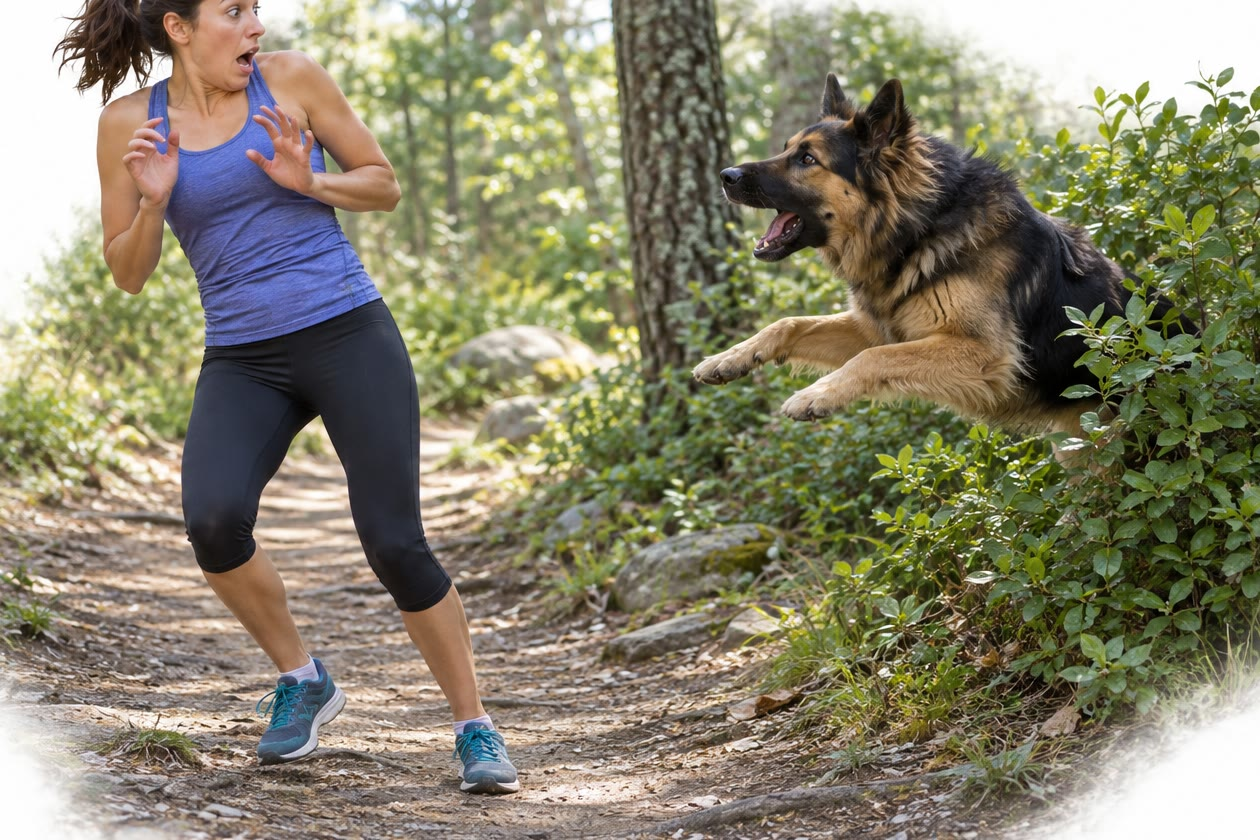
\includegraphics[width=0.6\linewidth]{images/book4/ai/b4-19-adrenaline-runner.jpg}

{\small La cascade à l'œuvre. Une frayeur libère de l'adrénaline depuis la
médullosurrénale~; en quelques secondes, le \omterm{def:b2:heart:anatomy}{cœur} s'emballe, le foie
déverse du glucose et les voies aériennes s'élargissent --- un seul
messager, plusieurs récepteurs, une amplification d'un facteur un
million dans chaque cellule.}
\end{omfigure}

\section{Les récepteurs intérieurs}

\begin{proposition}[Les récepteurs nucléaires]\label{prop:b2:cell-signalling:nuclear}
\index{recepteur nucleaire@récepteur nucléaire}\index{hormone steroide@hormone stéroïde}
Les stéroïdes, la thyroxine, l'acide rétinoïque et la vitamine D
diffusent à travers la membrane et se fixent sur des récepteurs du
cytosol ou du noyau qui sont eux-mêmes des \emph{\omterm{prop:b2:cell-differentiation:transcriptional}{facteurs de
transcription}}~: le complexe hormone--récepteur se fixe sur des séquences
d'ADN spécifiques et active ou réprime ses gènes cibles. La réponse est
lente --- des minutes à des heures pour fabriquer l'ARNm et la protéine
--- et durable~: le cortisol induit les enzymes de la néoglucogenèse pour
des heures, l'œstradiol construit la muqueuse utérine en quelques jours,
la testostérone fabrique du muscle en quelques semaines, la thyroxine
fixe le métabolisme de base de chaque cellule. Certains stéroïdes ont
aussi des actions rapides par des récepteurs de surface, et certaines
voies de surface atteignent aussi le noyau (la cascade des MAP kinases)~:
la distinction n'est donc pas absolue~; mais la règle demeure qu'un
messager liposoluble modifie ce qu'une cellule \emph{est} en modifiant
ses gènes, tandis qu'un messager hydrosoluble modifie ce qu'elle
\emph{fait} en modifiant ses enzymes.
\end{proposition}

\begin{omfigure}
\begin{tikzpicture}[every node/.style={font=\scriptsize}, >=stealth]
  \foreach \x/\t in {0/{hydrosolubles~: adrénaline, insuline, glucagon}, 7.4/{liposolubles~: cortisol, œstradiol, thyroxine}} \node[anchor=south, font=\scriptsize\bfseries] at (\x+2.6,3.4) {\t};
  % left: surface receptor
  \fill[omExo!30] (0,2.4) rectangle (5.2,2.8);
  \draw[thick, fill=omDef!40] (1.6,2.1) rectangle (2.3,3.1);
  \fill[omProp] (1.95,3.35) circle (0.1);
  \draw[->, thick] (1.95,2.1) -- (1.95,1.6) node[below, align=center] {seconds messagers,\\kinases~: enzymes\\commutées en secondes};
  \node[align=center] at (4.5,1.0) {change ce que\\la cellule fait};
  % right: nuclear receptor
  \begin{scope}[xshift=7.4cm]
    \fill[omExo!30] (0,2.4) rectangle (5.2,2.8);
    \fill[omProp] (1.5,3.35) circle (0.1);
    \draw[->, omProp] (1.5,3.25) -- (1.5,1.9);
    \draw[thick, fill=omThm!20] (1.5,1.5) ellipse (0.72 and 0.3); \node at (1.5,1.5) {récepteur};
    \draw[thick] (0.6,0.4) -- (4.6,0.4); \draw[thick] (0.6,0.25) -- (4.6,0.25); \node[below] at (2.6,0.2) {ADN~: gènes cibles activés ou réprimés, heures};
    \draw[->, thick] (1.5,1.2) -- (2.4,0.5);
    \node[align=center] at (4.0,1.4) {change ce que\\la cellule est};
  \end{scope}
\end{tikzpicture}

{\small Deux modèles. Un messager hydrosoluble agit à la surface et
modifie l'activité des enzymes en quelques secondes~; un messager
liposoluble entre, se fixe sur un récepteur qui est un \omterm{prop:b2:cell-differentiation:transcriptional}{facteur de
transcription}, et modifie l'expression des gènes en quelques heures.}
\end{omfigure}

\section{Un cas détaillé~: insuline, glucagon et consigne glycémique}

\begin{proposition}[Deux hormones et une consigne]\label{prop:b2:cell-signalling:glucose}
\index{insuline}\index{glucagon}\index{glycemie@glycémie}
Le glucose sanguin est maintenu vers \qty{5}{mmol/L} (\qty{0.9}{g/L})
par deux \omterm{def:b2:cell-signalling:kinds}{hormones} antagonistes des îlots pancréatiques. Après un repas,
la hausse du glucose est perçue par les cellules $\beta$ --- qui le
métabolisent, ferment un canal potassique à mesure que leur ATP
augmente, se dépolarisent, laissent entrer du calcium et libèrent de
l'\emph{insuline} --- et l'insuline, par son \omterm{prop:b2:cell-signalling:rtk}{récepteur à activité
tyrosine kinase}, fait absorber le glucose par les muscles et le tissu
adipeux (en déplaçant des transporteurs vers leurs membranes), le fait
stocker par le foie sous forme de glycogène et de graisse, et fait cesser
la combustion des graisses dans tous les tissus. Entre les repas, la
baisse du glucose laisse les cellules $\alpha$ libérer du
\emph{glucagon}, qui, par l'AMPc hépatique, dégrade le glycogène et
fabrique du glucose neuf à partir d'acides aminés~; l'adrénaline fait de
même, plus vite, en cas d'urgence, et le cortisol et l'\omterm{def:b2:cell-signalling:kinds}{hormone} de
croissance en quelques heures. Chaque \omterm{def:b2:cell-signalling:kinds}{hormone} est libérée en proportion
de l'écart qu'elle corrige~: une rétroaction négative à deux effecteurs,
un pour chaque sens, et une consigne défendue à un cinquième près. Le
cerveau, qui brûle \qty{120}{g} de glucose par jour et n'en stocke pas,
est l'organe que la boucle protège~; le diabète de type 1 est la perte
des cellules $\beta$, et son évolution sans traitement --- glucose à
\qty{20}{mmol/L}, graisses brûlées faute d'insuline, acide dans le \omterm{def:b2:blood-circulation:blood}{sang}
--- montre ce que devient la boucle privée d'un de ses bras.
\end{proposition}

\begin{omfigure}
\begin{tikzpicture}
\begin{axis}[
  width=0.82\linewidth, height=5.6cm,
  axis x line=bottom, axis y line=left,
  xmin=0, xmax=6, ymin=0, ymax=1.1,
  xlabel={heures après un repas}, ylabel={relatif au maximum},
  xlabel style={font=\small, at={(axis description cs:0.5,-0.12)}, anchor=north},
  ylabel style={font=\small},
  tick label style={font=\small}, xtick={0,1,2,3,4,5,6}, ytick={0,0.5,1},
  legend style={font=\scriptsize, at={(0.5,-0.28)}, anchor=north, draw=none, legend columns=3},
  clip=false,
]
\addplot[very thick, omDef, domain=0:6, samples=80] {0.55 + 0.45*exp(-((x-0.9)^2)/0.5) - 0.08*exp(-((x-4)^2)/2)};
\addlegendentry{glycémie (5 mmol/L à 0.55)}
\addplot[very thick, omThm, domain=0:6, samples=80] {0.15 + 0.85*exp(-((x-1.1)^2)/0.45)};
\addlegendentry{insuline}
\addplot[very thick, omProp, domain=0:6, samples=80] {0.75 - 0.5*exp(-((x-1.2)^2)/0.8) + 0.25*(1-exp(-x/5))*0.6};
\addlegendentry{glucagon}
\end{axis}
\end{tikzpicture}

{\small Glucose, insuline et glucagon après un repas. L'insuline augmente
avec le glucose et le fait redescendre~; lorsque le glucose retombe vers
la consigne, le glucagon augmente pour l'y maintenir.}
\end{omfigure}

\begin{example}[Vitesse, portée et coût des deux systèmes]\label{ex:b2:cell-signalling:compare}
L'adrénaline sanguine atteint toutes les cellules en une minute environ
(le temps de circulation) et agit pendant des minutes~; un influx
nerveux atteint sa cible en quelques millisecondes et agit pendant
quelques millisecondes. Une \omterm{def:b2:cell-signalling:kinds}{hormone} ne coûte presque rien par cellule
atteinte --- une nanomole répartie dans tout le corps --- mais ne peut pas
s'adresser à une seule cellule~; un nerf s'adresse exactement à une
cellule, mais doit construire et entretenir un fil jusqu'à elle.
L'organisme utilise les deux~: les nerfs sympathiques du
\cref{ch:b2:blood-pressure} agissent sur le \omterm{def:b2:heart:anatomy}{cœur} et les \omterm{def:b2:blood-circulation:vessels}{artérioles} en une
seconde, et la médullosurrénale, elle-même un ganglion sympathique
modifié, les relaie en déversant la même molécule dans le \omterm{def:b2:blood-circulation:blood}{sang} pour le
corps entier. Et à la synapse, les deux modèles se rejoignent, car un
\omterm{def:b2:cell-signalling:kinds}{neurotransmetteur} est un messager qui agit sur un récepteur par les
mêmes mécanismes --- un canal qui s'ouvre, une \omterm{prop:b2:cell-signalling:gpcr}{protéine G} qui commute ---
simplement sur vingt nanomètres au lieu d'un mètre.
\end{example}

\section{Exercices}

\begin{exercise}[$\star$]\label{exo:b2:cell-signalling:1}
Classer comme endocrine, paracrine, autocrine ou synaptique, et comme
hydrosoluble ou liposoluble~: l'insuline, le cortisol, l'acétylcholine à
une synapse, l'histamine dans une plaie, l'œstradiol, l'adrénaline de la
surrénale, le monoxyde d'azote de l'endothélium.
\end{exercise}

\begin{exercise}[$\star$]\label{exo:b2:cell-signalling:2}
Énumérer les étapes qui mènent de l'adrénaline sur la membrane d'une
cellule du foie au glucose dans le \omterm{def:b2:blood-circulation:blood}{sang}, et nommer l'interrupteur
d'arrêt de chaque étape.
\end{exercise}

\begin{exercise}[$\star$]\label{exo:b2:cell-signalling:3}
Comparer récepteurs de surface et \omterm{prop:b2:cell-signalling:nuclear}{récepteurs nucléaires}~: ce qui s'y
fixe, leur localisation, leur rapidité d'action, ce qu'ils modifient.
\end{exercise}

\begin{exercise}[$\star$]\label{exo:b2:cell-signalling:4}
Quels sont les trois \omterm{prop:b2:cell-signalling:gpcr}{seconds messagers} universels cités dans ce
chapitre, comment chacun est-il élevé, et comment chacun est-il
éliminé~?
\end{exercise}

\begin{exercise}[$\star\star$]\label{exo:b2:cell-signalling:5}
Un récepteur a une $K_d = \qty{2}{nmol/L}$. Calculer le taux d'occupation
à 0.2, 2, 20 et \qty{200}{nmol/L}. Une cellule double le nombre de ses
récepteurs~: qu'est-ce qui change, le taux d'occupation ou le nombre de
récepteurs occupés~?
\end{exercise}

\begin{exercise}[$\star\star$]\label{exo:b2:cell-signalling:6}
Une cascade comporte des étapes de gains 50, 200, 100 et 300. Calculer
l'amplification globale. Si l'\omterm{def:b2:cell-signalling:kinds}{hormone} est à \qty{1}{nmol/L} et que
\qty{1}{\%} des récepteurs ($10^{4}$ par cellule) sont occupés, combien
de molécules de produit la cellule fabrique-t-elle par seconde si le
gain de chaque étape est donné par seconde~?
\end{exercise}

\begin{exercise}[$\star\star$]\label{exo:b2:cell-signalling:7}
La toxine cholérique bloque la \omterm{prop:b2:cell-signalling:gpcr}{protéine G} stimulatrice dans son état lié
au GTP dans les cellules intestinales. Expliquer, étape par étape,
pourquoi le patient perd des litres de liquide par jour, et pourquoi
l'effet persiste des jours après la disparition des bactéries.
\end{exercise}

\begin{exercise}[$\star\star$]\label{exo:b2:cell-signalling:8}
Le calcium cytosolique passe de \qty{0.1}{} à \qty{1}{\micro mol/L} dans
une cellule de \qty{2000}{\micro m^3} lorsqu'un canal s'ouvre. Combien
d'ions calcium sont entrés~? Si un seul canal ouvert laisse passer
$10^{6}$ ions par seconde, combien de temps a-t-il fallu à un seul canal,
et pourquoi une cellule en ouvre-t-elle beaucoup à la fois~?
\end{exercise}

\begin{exercise}[$\star\star$]\label{exo:b2:cell-signalling:9}
L'insuline et le glucagon agissent tous deux sur le foie, l'une par une
tyrosine kinase, l'autre par l'AMPc. Expliquer comment la cellule
hépatique intègre les deux signaux, ce qui arrive au glycogène lorsque
les deux sont élevés, et pourquoi le rapport importe davantage que
chacun des deux taux.
\end{exercise}

\begin{exercise}[$\star\star\star$]\label{exo:b2:cell-signalling:10}
L'adrénaline élève l'AMPc d'une cellule du foie en \qty{5}{s} et la
production de glucose en \qty{30}{s}~; le cortisol élève les enzymes de
la néoglucogenèse du foie en \qty{4}{h}. À l'aide de la diffusion, de la
transcription (\qty{50}{} nucléotides par seconde sur un gène de
\qty{3000}{} nucléotides), de la traduction (\qty{5}{} acides aminés par
seconde sur une protéine de \num{500} résidus) et de la nécessité
d'accumuler des milliers de molécules d'enzyme, rendre compte des deux
échelles de temps.
\end{exercise}

\begin{exercise}[$\star\star\star$]\label{exo:b2:cell-signalling:11}
Une \omterm{def:b2:genome-diversification:mutation}{mutation} fait se dimériser, et donc signaler, un \omterm{prop:b2:cell-signalling:rtk}{récepteur à
activité tyrosine kinase} d'un facteur de croissance en l'absence de son
ligand. Prévoir le comportement de la cellule, expliquer pourquoi c'est
une étape fréquente des cancers, et dire ce que ferait un médicament qui
bloque le site de fixation de l'ATP de la kinase.
\end{exercise}

\begin{exercise}[$\star\star\star$]\label{exo:b2:cell-signalling:12}
«~Le système endocrinien diffuse~; le système nerveux câble.~» Discuter
les deux modèles du point de vue de la vitesse, de la portée, de la
spécificité et du coût, et dire où chacun est indispensable et où
l'organisme utilise les deux pour le même message.
\end{exercise}

\section{Problème~: une hormone du sang au gène}

\begin{problem}[{Problème du week-end --- l'adrénaline suivie de la glande
surrénale jusqu'au glucose d'une cellule du foie, avec le calcul de sa
concentration, du taux d'occupation de ses récepteurs, du gain de la
cascade et de sa chronologie, puis le cortisol suivi jusqu'à un gène, et
l'analyse de la boucle glycémique, jusqu'au taux d'occupation, à
l'amplification et au temps que met chaque hormone}]
\label{pb:b2:cell-signalling:1}
Données~: lors d'une frayeur, la médullosurrénale libère \qty{1}{nmol}
d'adrénaline dans \qty{5}{L} de \omterm{def:b2:blood-circulation:blood}{sang}~; la $K_d$ de l'adrénaline pour le
récepteur hépatique vaut \qty{1}{nmol/L}~; une cellule du foie
(\qty{5000}{\micro m^3}) porte $2\times 10^{4}$ récepteurs. Gains de la
cascade par seconde d'activation~: récepteur $\to$ \omterm{prop:b2:cell-signalling:gpcr}{protéine G} 20,
\omterm{prop:b2:cell-signalling:gpcr}{protéine G} $\to$ AMPc 100 (le nombre de cycles de la cyclase pendant les
3 secondes de vie de la \omterm{prop:b2:cell-signalling:gpcr}{protéine G}), AMPc $\to$ kinase A 1
(stœchiométrique), kinase A $\to$ phosphorylase kinase 50, $\to$
phosphorylase 50, $\to$ glucose 1000. Le foie contient \qty{100}{g} de
glycogène. Cortisol~: transcription à \qty{50}{} nucléotides par seconde
sur un gène de \qty{4000}{} nucléotides, traduction à \qty{5}{} résidus
par seconde sur une enzyme de \num{600} résidus, \num{20} ribosomes par
ARNm, \num{100} ARNm produits par heure, un effet qui exige $10^{5}$
molécules d'enzyme.

\medskip
\noindent\textbf{Partie I --- L'arrivée de l'\omterm{def:b2:cell-signalling:kinds}{hormone}.}
\begin{enumerate}
  \item Calculer la concentration plasmatique d'adrénaline après la
        libération, en négligeant son élimination.
  \item Calculer le \omterm{thm:b2:cell-signalling:occupancy}{taux d'occupation des récepteurs} et le nombre de
        récepteurs occupés par cellule du foie.
  \item L'adrénaline est éliminée avec une demi-vie de \qty{2}{min}.
        Quelles sont sa concentration et le taux d'occupation au bout de
        \qty{6}{min}~?
  \item Combien de temps l'adrénaline met-elle pour aller de la
        surrénale au foie, sachant que le temps de circulation est
        d'environ une minute~? Pourquoi le nerf sympathique du foie
        agit-il plus vite~?
  \item Une cellule porte $2\times 10^{5}$ récepteurs de même $K_d$~:
        qu'est-ce qui change~?
  \item Pourquoi $K_d$ est-elle accordée à la concentration circulante ---
        que ferait un récepteur de $K_d = \qty{1}{\micro mol/L}$ face à
        une \omterm{def:b2:cell-signalling:kinds}{hormone} nanomolaire~?
\end{enumerate}

\medskip
\noindent\textbf{Partie II --- La cascade.}
\begin{enumerate}[resume]
  \item Calculer le gain global d'un récepteur occupé en molécules de
        glucose par seconde.
  \item Calculer le nombre de molécules d'AMPc fabriquées par la cellule
        pendant la première seconde, et la concentration qu'elles
        atteignent dans son volume.
  \item Calculer la production de glucose d'une cellule du foie par
        seconde au taux d'occupation de la question 2, et par minute.
  \item Le foie compte $2\times 10^{11}$ cellules. Calculer la
        production que prédisent les gains, en grammes par minute, et la
        comparer aux \qty{5}{g/min} réellement observés. Qu'est-ce qui
        limite la production réelle~?
  \item Combien de temps les \qty{100}{g} de glycogène dureraient-ils à
        ce rythme~? Pourquoi ne s'épuisent-ils pas lors d'une frayeur~?
  \item Nommer l'interrupteur d'arrêt de chaque étape amplificatrice et
        dire lequel agit le plus vite.
  \item Un inhibiteur de la phosphodiestérase (la caféine) est présent.
        Prévoir l'effet sur la cascade et sur la production de glucose.
\end{enumerate}

\medskip
\noindent\textbf{Partie III --- Du cortisol au gène.}
\begin{enumerate}[resume]
  \item Calculer le temps nécessaire pour transcrire un ARNm.
  \item Calculer le temps nécessaire pour traduire une molécule
        d'enzyme, et le nombre de molécules d'enzyme par ARNm et par
        heure (chaque ARNm vivant une heure, les ribosomes démarrant l'un
        après l'autre).
  \item Calculer le nombre de molécules d'enzyme fabriquées par heure à
        partir des \num{100} ARNm, et le temps nécessaire pour atteindre
        $10^{5}$.
  \item Ajouter le temps nécessaire au cortisol pour entrer, se fixer et
        atteindre l'ADN (quelques minutes), et expliquer les \qty{4}{h}
        observées.
  \item Pourquoi l'organisme n'utiliserait-il pas une cascade comme celle
        de l'adrénaline pour la tâche du cortisol, et pourquoi pas le
        mécanisme du cortisol pour une frayeur~?
  \item Le cortisol augmente aussi le nombre de récepteurs à l'adrénaline
        des cellules du foie. Expliquer comment une \omterm{def:b2:cell-signalling:kinds}{hormone} lente peut
        amplifier une \omterm{def:b2:cell-signalling:kinds}{hormone} rapide, et ce que cela fait à la courbe
        d'occupation de l'\omterm{def:b2:cell-signalling:kinds}{hormone} rapide.
\end{enumerate}

\medskip
\noindent\textbf{Partie IV --- La boucle.}
\begin{enumerate}[resume]
  \item Après un repas, le glucose passe de 5 à \qty{8}{mmol/L}. Décrire
        la réponse de la cellule $\beta$, du glucose à la libération
        d'insuline, en nommant le couplage.
  \item L'insuline agit par une tyrosine kinase, le glucagon par l'AMPc.
        Expliquer pourquoi une même cellule peut obéir aux deux, et
        comment les enzymes du glycogène du foie sont réglées par leur
        rapport.
  \item Un patient n'a plus de cellules $\beta$. Prévoir sa glycémie à
        jeun et après un repas, et expliquer pourquoi les graisses sont
        brûlées et de l'acide apparaît.
  \item L'insuline injectée n'est soumise à aucune rétroaction. Expliquer
        le danger d'une course inhabituellement longue avec une dose
        habituelle.
  \item Comparer la boucle glycémique au \omterm{def:b2:blood-pressure:baroreflex}{baroréflexe} du
        \cref{ch:b2:blood-pressure}~: capteur, effecteurs, gain, vitesse.
  \item Énoncer le résultat~: le taux d'occupation de l'adrénaline après
        sa libération, le gain de la cascade, la production de glucose du
        foie et le temps que met le cortisol.
\end{enumerate}
\end{problem}
